\documentclass{article}
\usepackage{xspace}
\usepackage{graphicx}
\usepackage{amsmath}

\title{Technical report for Workshop 1.5 data analysis}
\author{S.~Sinclair}

\newcommand{\emerge}{\textsc{[E]merge}\xspace}
\newcommand{\todo}[1]{\emph{To do: #1}}
\newcommand{\func}[1]{\texttt{#1}}

\begin{document}
\maketitle

\begin{abstract}
This document presents a summary of analysis techniques used to
interpret the data collected during the \emerge ``Workshop 1.5''
recording session, which took place Apr. 30, 2011.
\end{abstract}

\section{Overview}

\todo{Description of data collection (data format, metadata, time handling, etc.)}

10 Hz, range 10 bit.  8 minibees were recorded.  Current video frame,
time of data reception was recorded.  Video was tagged manually
afterwards.

\todo{Overview of analysis approach (features, prediction)}

\todo{List of features}

\begin{itemize}
  \item Amplitude (root mean square).
  \item Frequency and periodicity.
    \begin{itemize}
    \item Zero-crossing analysis.
    \item Autocorrelation.
    \end{itemize}
  \item Visualized range/variance---analysis of linear regression
    angle and variance in plots of data.
  \item Covariance/correlation analysis.
  \item Max/min over various window sizes.
  \item Jerk.
\end{itemize}

\todo{Comparison methods}

\begin{itemize}
  \item Neural net prediction performance
\end{itemize}

\section{Features}

Features were analysed in Scientific Python (SciPy) and Matlab
environments, and this document will make reference to functions in
these applications.

Most features are based on windows of the signal.  We will use the
notation $x_w$ to denote window $w$ of signal $x$.

Windows are $n$ samples in length and separated by a hopsize $h$, such
that
\begin{align}
x_w &= \left[\begin{array}{cccc}x(hw)&x(hw+\tau)&\dots&x(hw + n\tau)\end{array}\right],
\end{align}
with a sample rate of $\tau.$
Windows may also be referred to as ``blocks''.

\subsection{Amplitude (root mean square)}

The accelerometer signal is a 3-vector in Cartesian coordinates, from
which a magnitude can be taken by converting to polar coordinates:

\begin{align}
\textrm{mag}(x) &= \sqrt{x_1^2 + x_1^2 + x_1^2}
\end{align}

The amplitude of the signal is then determined on a block-wise basis
by method of root mean square (RMS), calculated as,
\begin{align}
\textrm{RMS}(m_w) &= \sqrt\frac{\sum^n_{i=1}{m_w(i)}}{n},
\end{align}
where $m_w$ is window $w$ of the magnitude signal $m$.

\subsection{Frequency and periodicity}

When working with low-frequency data such as gesture signals, it is
not necessarily possible to rely on frequency-domain approaches such
as the Fourier transform for fundamental frequency ($f_0$) estimation
due to poor resolution in the low-frequency range.

Instead, we pursued two time-domain methods, zero-crossing analysis
and autocorrelation.

\subsubsection{Zero-crossing analysis}

For a signal with low noise and few harmonics, it can be possible to
determine its frequency by determining the times at which the signal
crosses zero, and differentiating these to calculate a period size.

We calculated zero crossings of a high-pass magnitude signal.  That
is, the magnitude signal was low-pass filtered to determine a running
mean, and the original signal then subtracted this to produce a signal
oscillating around zero.

Zero-crossings in the positive direction were detected and linear
interpolation was used to find the sub-sample position.
Frequency was then calculated by dividing the period.

The notion of ``periodicity'' was taken to mean the opposite of the
deviation from the mean frequency.
That is to say, a signal whose frequency is changing often should be
thought of as having low periodicity, and a signal with a fairly
constant frequency should be thought of as having high periodicity.
Periodicity was therefore calculated by taking the standard deviation
of a high-pass frequency signal and subtracting this from the maximum.

In general neither frequency nor periodicity determined by
zero-crossings seemed to be a successful indicator of gesture.
This is perhaps due to the low sampling rate of the data and the
presence of likely aliasing which would introduce high-frequency
artifacts, so it may be useful to try this method on better-sampled
data.

\subsubsection{Autocorrelation}

\begin{figure}
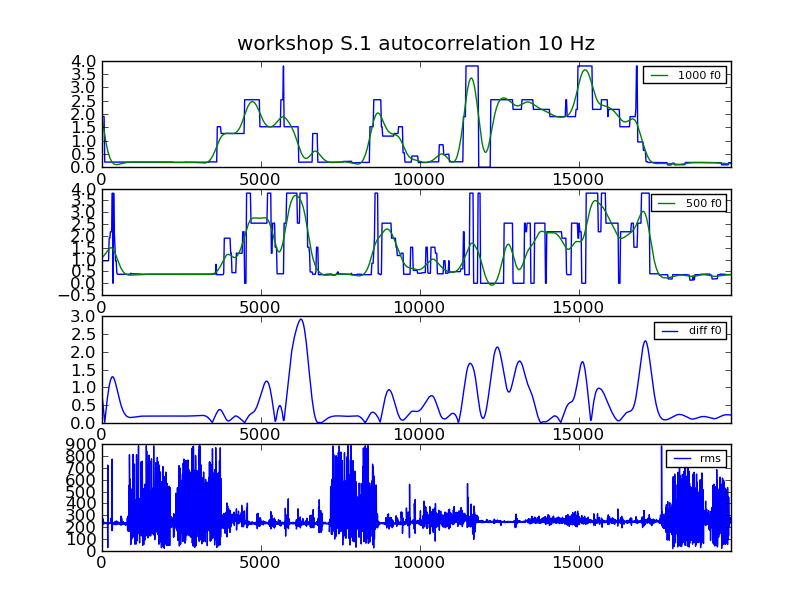
\includegraphics[width=0.5\textwidth]{images/workshop_autocorr_10hz_m1.png}
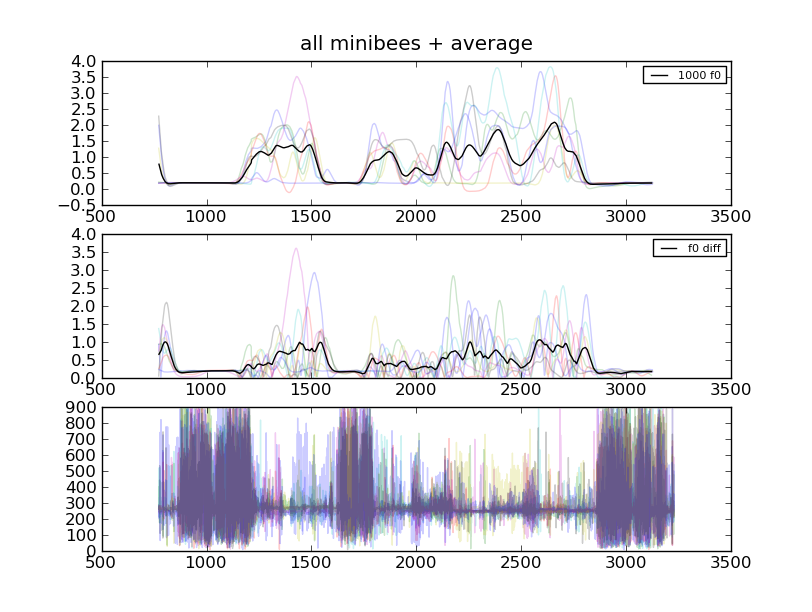
\includegraphics[width=0.5\textwidth]{images/workshop_all_autocorr_f0_10hz.png}
\caption{(Left) Autocorrelation $f_0$ estimation for two window sizes
  (1000 points, 500 points) for Minibee~1, and the difference between
  them.  (Right) Average of same over all minibees.}
\label{autof0}
\end{figure}

Autocorrelation is often used for low-frequency $f_0$ estimation.
It is the process of comparing a signal with a delayed version of
itself to find periodic patterns.

Correlation was calculated by SciPy function \func{correlate}, Matlab
function \func{corr}; autocorrelation by providing the same signal to
the two arguments.
This produces a symmetric triangular shape with peaks indicating delay
values of high correlation.

The autocorrelation vector can be calculated block-wise and plotted,
producing a spectrogram-like image. \todo{figure}

For each window, the horizontal location of the first peak to the
right of the triangle apex was found, representing a single period.
From this, frequency was calculated.

It was found that the $f_0$ estimation tended to vary quite a lot
depending on the window size used.
It is likely that the peak picking algorithm for analysis of the
correlation vector should be more intelligent to avoid choosing the
wrong harmonic, perhaps using likelihood based on surrounding blocks.
Results of two window sizes (1000 points and 500 points) can be seen
in Fig.~\ref{autof0}.

This was performed for each minibee, and the average was taken.  It
became clear that the $f_0$ estimation was quite steady during periods
of high activity, but gave a significant amount of variance during
low-activity periods.

Due to this variance in the frequency estimation, it is not yet clear
how well this can be used to determine periodicity.  However, from
visualizing the autocorrelation-gram, it is perhaps more likely that
using the full correlation vector, or the relative locations and
heights of significant peaks, could produce a more salient indication
of gesture characteristics.

\subsection{Visualized range/variance}

Plotting linear regression angle and deviation size. (Joe)

\subsection{Covariance/correlation analysis}

\begin{figure}
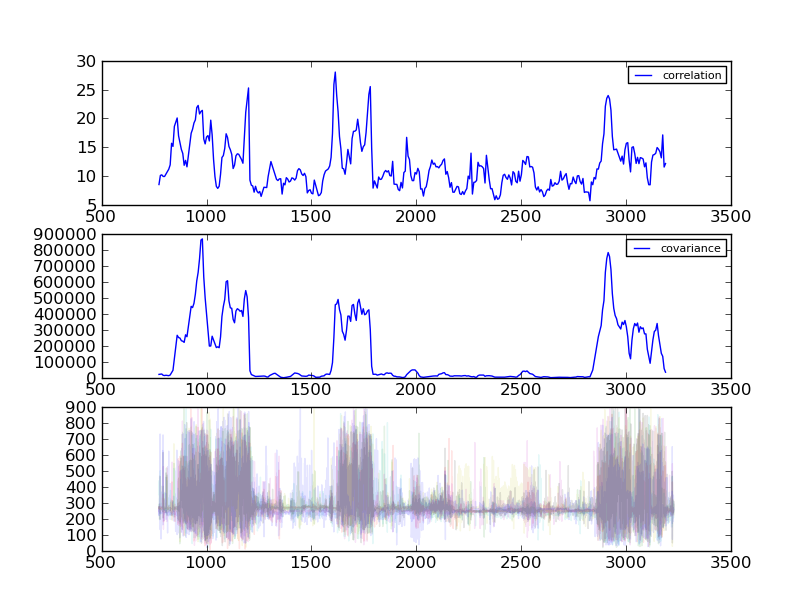
\includegraphics[width=0.5\textwidth]{images/corr_cov.png}
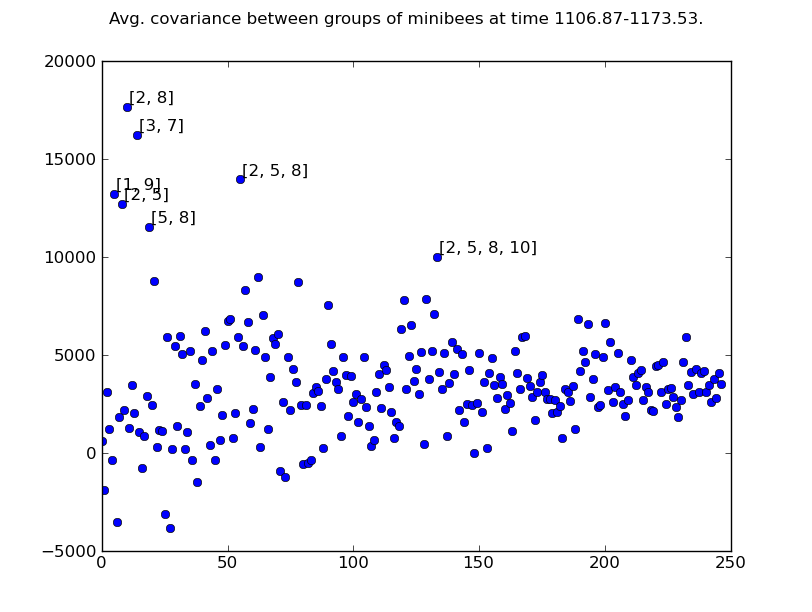
\includegraphics[width=0.5\textwidth]{images/cov_groups_1106.png}
\caption{(Left) Sum of correlation and covariance matrices across all
  minibees.  Covariance is an excellent indicator of common activity.
  (Right) Average covariance across pairs within all possible
  sub-groups of minibees for a window at time 1106--1173.  Some
  outliers are identified.}
\label{covgroups}
\end{figure}

Correlation and covariance across all minibees was explored as a means
to estimate relationships between accelerometer activity.
SciPy functions \func{correlate} and \func{cov} produce a matrix that
indicates the corresponding relationship between each pair of signals.
This was computed block-wise on the accelerometer magnitude and summed
to produce graphs seen on the left of Fig.~\ref{covgroups}.

It is clear that the total covariance shows presence or non-presence
of common group activity, at least for high-energy activity.
It is possible that correlation may provide useful information for
low-energy activities, though it may be difficult to distinguish from
noise.
This has not yet been tested.

Next, it was attempted to identify groups within the minibee data
which had particularly high covariance.
The powerset of the list of minibees was computed, producing 247
sub-groups.
For each of group, all pair combinations' covariance values were averaged.

The right side of Fig.~\ref{covgroups} shows the result for one window
during the first activity period, where the horizontal ordering has
smaller groups to the left and larger groups to the right of the
graph.
Therefore more averaging of the covariance occurs from left to right.
Some outliers are identified in the upper-left quadrant of the graph.
Of these, it is interesting that some groups do not intersect.
For example, (3,7), (1,9) and (2,5,8) seem to be covarying
within-group but not between each other.

\subsection{Max/min over various window sizes}

(Sofian)

\subsection{Jerk}

(Sofian)

\section{Comparison methods}

\subsection{Neural net prediction}

Fig.~\ref{fig:predresults} shows error in the prediction using RMS and
zero-crossing-derived frequency and periodicity.

(Steve)

\begin{figure}
\centerline{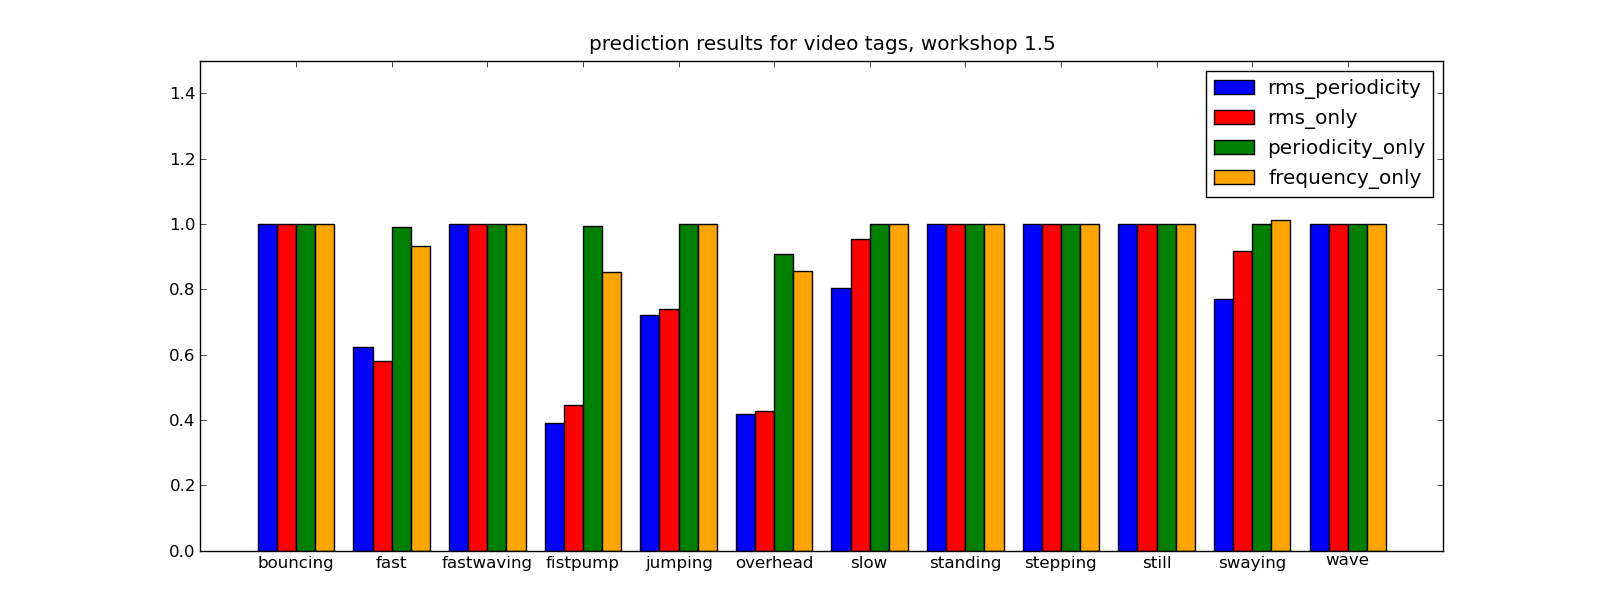
\includegraphics[width=\textwidth]{images/predictionresults.png}}
\caption{Ability of RMS, zero-crossing periodicity and frequency
  features to predict the video tags.  1 indicates 100\% error, zero
  indicates no error.  It can be seen that RMS seems to basically just
  predict activity; periodicity and frequency are not contributing.}
\label{fig:predresults}
\end{figure}

\end{document}
